\chapter{Progettazione}

Nella fase di progettazione, si sono fatte alcune assunzioni sull'ambiente, sul drone e sulle altre entità coinvolte durante la fase di simulazione.
In particolare, tali assunzioni riguardano le caratteristiche principali dell'ambiente e delle entità in esso coinvolte.

\section{Progettazione dell'ambiente}

L'ambiente che viene preso in esame dipende dallo scenario considerato per la simulazione della missione.
Esso rappresenta un'area bidimensionale strutturata e limitata, in cui lo spazio ed il tempo risultano entrambi discretizzati.

Lo spazio è simulato attraverso una griglia di \textit{NxM} celle quadrate, dette \textit{patch}, di lato \textit{S}. 
Il tempo è discretizzato in una sequenza di intervalli temporali di durata \textit{T} detti \textit{tick} definiti come:
\begin{equation*}
    t_0 + T, t_0 + 2T, \dots, t_0 + NT
\end{equation*}

L'ambiente simulato contiene i seguenti elementi: 
\begin{itemize}
    \item \textit{Droni};
    \item \textit{Target};
    \item \textit{Ostacoli};
    \item \textit{Feromoni digitali};
\end{itemize}

La figura \ref{elementi_ambiente} mostra una rappresentazione semplificata dell'ambiente di simulazione con gli elementi sopra descritti.

Nell'ambiente, un singolo UAV è rappresentato da un disco con un punta di freccia interna. 
La punta indica la direzione del drone. 
Ostacoli e target, solitamente, coprono diverse celle.
In figura, ogni cella in cui è presente un ostacolo è nera, mentre ogni cella-target è colorata. 
Come abbiamo già precedentemente accennato, un target può assumere diversi stati: in questo caso un target \textit{not found} è rappresentato da una cella rossa, un target \textit{found} da una cella verde e con una cella gialla, infine, un target \textit{executed}.
L'intensità del colore di bersaglio, quando applicabile (ad esempio, fuoco, gas, ecc.), rappresenta la quantità/presenza del target. 
Infine, una traccia feromonica è indicata da un gruppo di cellule grigie, dove la scala di grigio varia in base all'intensità dei feromoni.

\begin{figure}[H] 
    \captionsetup{justification=centering, margin=2cm, font=footnotesize}
    \begin{center}
    \makebox[\textwidth]{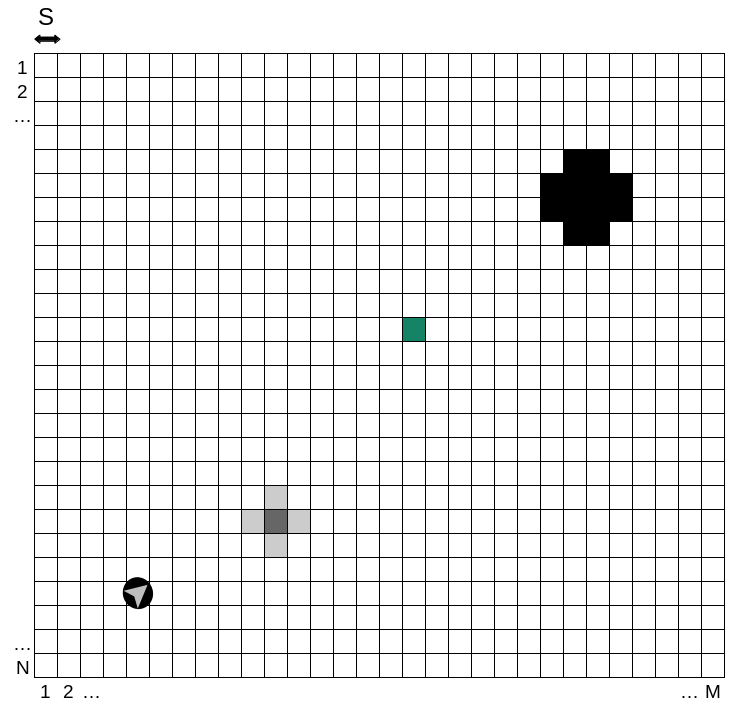
\includegraphics[width=0.4\paperwidth]{img/elementi_ambiente.png}}
    \end{center}
    \caption{Definizione dell'ambiente simulato: (da sinistra a destra) drone, feromone, target ed ostacolo.}
    \label{elementi_ambiente}
\end{figure}

Si assumano, per semplicità i seguenti valori:
\begin{itemize}
    \item S = 1 metro;
    \item T = 1 secondo; 
\end{itemize}

I valori sopra riportati, naturalmente, possono variare in base alla missione ed allo scenario in cui essa si svolge.
In questo caso, l'assunzione è necessaria per una conversione immediata da metri a numero di patch e da secondi a tick.

Supponendo di avere una patch di lato \textit{S} diverso da un metro, può essere sfruttata la seguente formula di conversione, per determinare il numero di patch a cui corrisponde un metro:

\begin{equation}
    \label{m_patches}
    1 \; m = \frac{1}{S} \; patches
\end{equation}

Allo stesso modo, si può determinare a quanti tick corrisponde un secondo:

\begin{equation}
    \label{sec_ticks}
    1 \; s = \frac{1}{T} \; ticks
\end{equation}

Dalle relazioni \ref{m_patches} e \ref{sec_ticks} è possibile determinare la formula di conversione da \textit{m/s} a \textit{patches/tick}:

\begin{equation*}
    1 \; m/s = (\frac{1}{S})(\frac{1}{T}) \; patches/tick 
\end{equation*}

Ad ogni tick, il drone effettua rilevamenti di ostacoli, target e feromoni vicini alla sua posizione ed esegue regole comportamentali precise.
Lo sciame di droni si muove separatamente, organizzato in diversi flock.

Il blocco fondamentale dello spazio discretizzato simulato è rappresentato dalla cella.
Ogni cella (denominata anche patch) ha delle coordinate \textit{x-y} nello spazio bidimensionale e può contenere un target o un ostacolo.
Una caratteristica fondamentale del simulatore è la possibilità di prenotare una patch: tale strategia, infatti, è pensata nel caso in cui è previsto un meccanismo di \textit{collision avoidance}, come nel caso dell'algoritmo SCIADRO.

Per illustrare la struttura di un oggetto \textit{patch}, consideriamo la cella come una classe.
Nella figura \ref{classe_patch} è possibile osservare tale struttura.

\begin{figure}[H] 
    \captionsetup{justification=centering, margin=2cm, font=footnotesize}
    \begin{center}
    \makebox[\textwidth]{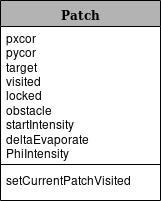
\includegraphics[width=0.2\paperwidth]{img/classe_patch.png}}
    \end{center}
    \caption{Struttura della classe Patch.}
    \label{classe_patch}
\end{figure}

\section{Elemento ostacolo}

Un ostacolo è un elemento che ostruisce il passaggio di un UAV. 
Esso ha una posizione statica e occupa una cella all’interno dell’ambiente di esplorazione. 
L’ostacolo non può essere attraversato dal drone e rappresenta la base per modellare diversi tipi di strutture come, ad esempio, alberi, costruzioni, ecc.

\section {Elemento target} \label{elemento_target}

Un target è un elemento collocato, all'istante \textit{t}, in una determinata posizione dell’ambiente di simulazione sconosciuta ai droni. 
La struttura di un target dipende da cosa si vuole modellare, in accordo con il task della missione:

\begin{itemize}
    \item \textit{Rilevamento di sostanze}, come un gas o un liquido tossico: in questo caso gli elementi sono modellati attraverso una distribuzione gaussiana di target, con media in corrispondenza della sorgente;
    \item \textit{Identificazione di oggetti}, come ad esempio mine anti-uomo: in questo caso il target è modellato come una singola cella;
    \item \dots
\end{itemize}

Lo stato di un target è identificato dalla variabile \textbf{target.state}, che può assumere i seguenti valori:

\begin{itemize}
    \item \textit{Found};
    \item \textit{Not found};
    \item \textit{Executed}.
\end{itemize}

Perché un target venga lavorato, dev'essere raggiunto da un numero minimo di agenti: questo parametro può essere configurato prima dell'avvio della simulazione e dipende dalla singola missione.

\begin{figure}[H] 
    \captionsetup{justification=centering, margin=2cm, font=footnotesize}
    \begin{center}
    \makebox[\textwidth]{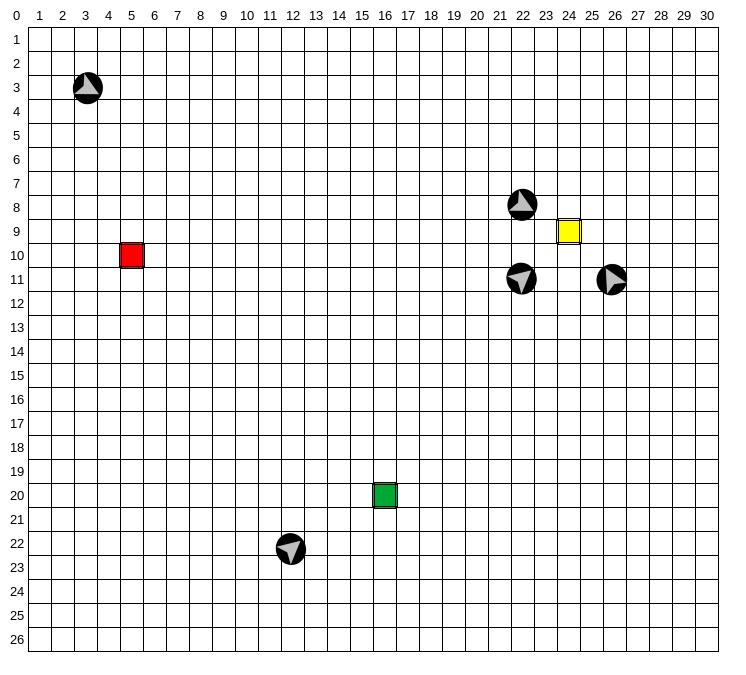
\includegraphics[width=0.4\paperwidth]{img/tipi_target.png}}
    \end{center}
    \caption{Stati di un target: (da sinistra a destra) \textit{Not found, Found, Executed}.}
    \label{tipi_target}
\end{figure}

La struttura della classe \textit{Target} è illustrata in figura \ref{classe_target}.
\begin{figure}[H] 
    \captionsetup{justification=centering, margin=2cm, font=footnotesize}
    \begin{center}
    \makebox[\textwidth]{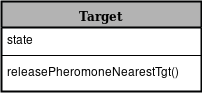
\includegraphics[width=0.2\paperwidth]{img/classe_target.png}}
    \end{center}
    \caption{Struttura della classe Target.}
    \label{classe_target}
\end{figure}

\section {Elemento UAV}

L'UAV è l'elemento in grado di muoversi in modo continuo all’interno dello spazio bidimensionale di ricerca con l’obiettivo principale di scoprire nuovi target. 
Inoltre, il drone deve evitare di scontrarsi con gli ostacoli o con altri droni e, insieme a loro, deve coordinarsi e completare il processo di scoperta dei target entro il tempo di autonomia, usando meccanismi di comunicazione diretta o indiretta, in base all’algoritmo integrato nel simulatore. 

Gli scontri e le collisioni con altri droni e con gli ostacoli sono, naturalmente, simulati. 
Per questo motivo, a partire dalla fase di progettazione, questi eventi possono essere denominati “sovrapposizioni tra droni e droni” e “sovrapposizioni tra droni e ostacoli”, rispettivamente. 
Si deve notare che il sensing potrebbe essere influenzato dalla velocità del drone. 
Esiste una velocità massima per cui la performance della tecnologia di sensing non risulta influenzata dalla velocità del drone: tale velocità è denominata velocità di crociera e risulta minore della velocità massima.

\section {Algoritmo bioispirato}

Alcune caratteristiche degli elementi presenti nel simulatore, come la struttura del drone o del feromone digitale, dipendono dall'algoritmo integrato all'interno dell'ambiente di simulazione.
Nella sezione successiva ci soffermeremo sulle metaeuristiche della strategia \textit{Sciadro}.
Successivamente, invece, prenderemo in esame gli elementi utilizzati nel gruppo di algoritmi analizzati precedentemente: \textit{FTS}, \textit{PSO} e \textit{ABC}.

\subsection{SciaDro}

In questa sezione entreremo nel dettaglio della progettazione dei vari elementi introdotti nel capitolo \ref{analisi} (\textit{Analisi}), quali il drone ed i vari meccanismi di flocking, collision avoidance e stigmergia.

\subsubsection{Progettazione del drone}

Il drone può essere modellato come un cerchio in movimento nello spazio bidimensionale. 
I parametri associati al drone dipendono dalle sue caratteristiche fisiche e architetturali. 
Lo stato del drone è caratterizzato da:

\begin{itemize}
    \item Posizione nell’ambiente (\textbf{drone.x} e \textbf{drone.y});
    \item Numero di droni vicini nello sciame (\textbf{drone.flockmates});
    \item Velocità di crociera (\textbf{drone.cruisingSpeed});
    \item Velocità corrente (\textbf{drone.speed});
    \item Direzione corrente (\textbf{drone.heading});
    \item Velocità angolare corrente (\textbf{drone.angularSpeed});
    \item Autonomia (\textbf{drone.endurance}).
\end{itemize}
Il drone esegue azioni al fine di:

\begin{enumerate}
    \item Evitare ostacoli
    \begin{itemize}
        \item Collision avoidance
    \end{itemize}
    \item Coordinarsi con gli altri droni attraverso il meccanismo di flocking
    \begin{itemize}
        \item Separate
        \item Align
        \item Cohere
    \end{itemize}
    \item Rilasciare il feromone
    \item Muoversi nell’ambiente per ricercare i targets
    \begin{itemize}
        \item Movement
        \item Accelerate
        \item Decelerate
    \end{itemize}
\end{enumerate}

Al fine di rilevare il target, è stato necessario inserire un codice di sensing. L’area del cono di sensing dipende prevalentemente dal tipo di sensore. 

Per le ragioni sopra menzionate, tutti questi parametri devono essere fissati prima di avviare la simulazione.

\begin{figure}[H] 
    \captionsetup{justification=centering, margin=2cm, font=footnotesize}
    \begin{center}
    \makebox[\textwidth]{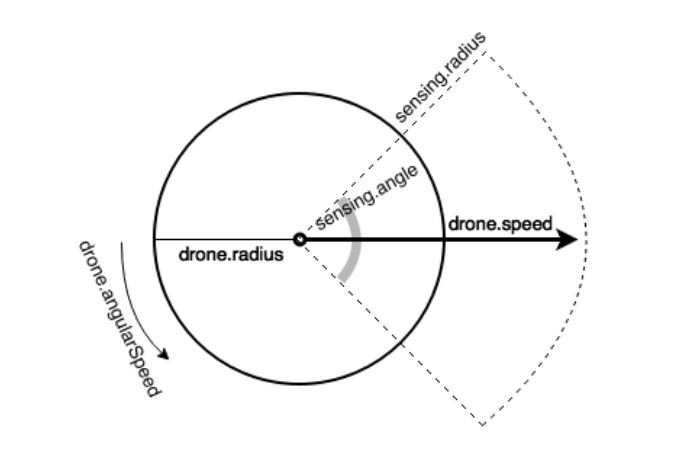
\includegraphics[width=0.4\paperwidth]{img/modello_parametrico_drone.png}}
    \end{center}
    \caption{Modello parametrico del drone.}
    \label{modello_drone}
\end{figure}

La seguente tabella riassume i parametri strutturali che caratterizzano il drone.
\begin{table}[H]
    \centering
    \begin{tabular}{|l|l|c|}
    \hline
    \textbf{Parametro}       & \textbf{Definizione}       & \textbf{Unità di misura}   \\ \hline
    drone.radius             & Raggio fisico              & (m)                        \\ \hline
    sensing.radius           & Raggio di sensing          & (m)                        \\ \hline
    sensing.angle            & Angolo di sensing          & (gradi)                    \\ \hline
    drone.cruisingSpeed      & Velocità di crociera       & (m/s)                      \\ \hline
    drone.speedMax           & Velocità massima           & (m/s)                      \\ \hline
    drone.speed              & Velocità corrente          & (m/s)                      \\ \hline
    drone.acceleration       & Accelerazione              & (m/s\textsuperscript{2})   \\ \hline
    drone.deceleration       & Decelerazione              & (m/s\textsuperscript{2})   \\ \hline
    drone.endurance          & Autonomia                  & (minuti)                   \\ \hline
    drone.heading            & Direzione corrente         & (gradi)                    \\ \hline
    drone.accelerationAng    & Accelerazione angolare     & (rad/s\textsuperscript{2}) \\ \hline
    drone.decelerationAng    & Decelerazione angolare     & (rad/s\textsuperscript{2}) \\ \hline
    drone.velocityAngularMax & Velocità angolare massima  & (rad/s\textsuperscript{2}) \\ \hline
    drone.angularSpeed       & Velocità angolare corrente & (rad/s\textsuperscript{2}) \\ \hline
    \end{tabular}
    \caption{Parametri strutturali del drone.}
\end{table}

Ad ogni ciclo di aggiornamento, il drone assume una posizione specifica nello spazio di ricerca, descritta da una coppia di coordinate.
Esso può essere equipaggiato con uno o più sensori e può muoversi sia in modo longitudinale che rotazionale.
Il drone, inoltre, è anche in grado di rilevare i target e di rilasciare impronte di feromone per la comunicazione indiretta con gli altri UAV.

\begin{figure}[H] 
    \captionsetup{justification=centering, margin=2cm, font=footnotesize}
    \begin{center}
    \makebox[\textwidth]{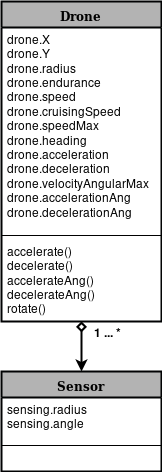
\includegraphics[width=0.2\paperwidth]{img/classe_drone.png}}
    \end{center}
    \caption{Struttura della classe Drone.}
    \label{classe_drone}
\end{figure}

\subsubsection{Progettazione del flocking}

Di seguito si illustra la progettazione del meccanismo di flocking descritto nella fase di analisi. 
Il drone distingue tre diverse aree di prossimità: l’area di separazione (\textit{separate}), l’area di allineamento (\textit{align}) e l’area di coesione (\textit{cohere}). 
Ciascuna di tali aree ha uno specifico raggio ed è associata ad uno specifico comportamento del drone.
Le tre aree di prossimità hanno in comune l’angolo \textbf{drone.flocking.angle}.

\begin{figure}[H] 
    \captionsetup{justification=centering, margin=2cm, font=footnotesize}
    \begin{center}
    \makebox[\textwidth]{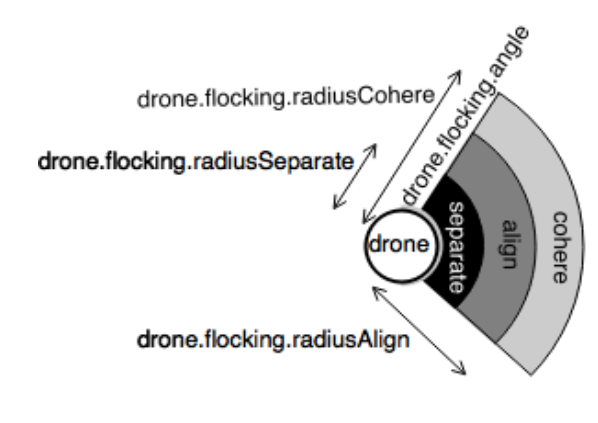
\includegraphics[width=0.4\paperwidth]{img/aree_flocking.png}}
    \end{center}
    \caption{Aree del meccanismo di flocking.}
    \label{aree_flocking}
\end{figure}

I parametri illustrati nella figura \ref{aree_flocking}, sono analizzati in dettaglio nella seguente tabella.
\begin{table}[H]
    \centering
    \resizebox{\textwidth}{!}{%
    \begin{tabular}{|l|l|c|}
    \hline
    \textbf{Parametro}             & \textbf{Definizione}                                                                    & \textbf{Unità di misura} \\ \hline
    drone.flocking.angle           & Angolo di visione del flock                                                             & (gradi)                  \\ \hline
    drone.flocking.radiusCohere    & Raggio di coesione $\in$ (drone.flocking.radiusAlign, +$\infty$)                            & (m)                      \\ \hline
    drone.flocking.maxCohereTurn   & Angolo di rotazione massimo nel meccanismo di coesione                                  & (gradi)                  \\ \hline
    drone.flocking.radiusAlign     &\begin{tabular}[c]{@{}l@{}}Raggio di allineamento $\in$ (drone.flocking.radiusSeparate, \\ drone.flocking.radiusCohere]\end{tabular} & (m)                      \\ \hline
    drone.flocking.maxAlignTurn    & Angolo di rotazione massimo nel meccanismo di allineamento                              & (gradi)                  \\ \hline
    drone.flocking.radiusSeparate  & Raggio di separazione $\in$ (drone.collisionVision, +$\infty$)                              & (m)                      \\ \hline
    drone.flocking.maxSeparateTurn & Angolo di rotazione massimo nel meccanismo di separazione                               & (gradi)                  \\ \hline
    drone.flocking.wiggleVar       & Numero casuale $\in$ (0,N)                                                                   & (adimensionale)          \\ \hline
    \end{tabular}%
    }
    \caption{Parametri strutturali del flocking.}
    \label{tabella_flocking}
\end{table}

\paragraph{Comportamento separate:} se un drone si trova all'interno dell'area identificata dal raggio \textbf{drone.flocking.radiusSeparate}, allora viene attivato il meccanismo di separazione, ovvero una rotazione che porta il drone a separarsi dal resto del flock.
Tale rotazione è limitata all'angolo \textbf{drone.flocking.maxSeparateTurn}.

\begin{figure}[H] 
    \captionsetup{justification=centering, margin=2cm, font=footnotesize}
    \begin{center}
    \makebox[\textwidth]{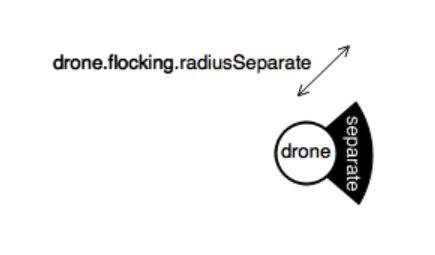
\includegraphics[width=0.4\paperwidth]{img/separate.png}}
    \end{center}
    \caption{Area di riferimento per il comportamento \textit{Separate}.}
    \label{separate}
\end{figure}

\paragraph{Comportamento aling:} il drone verifica la presenza di altri droni nell'area di align e ruota di un angolo \textbf{drone.flocking.alignAngle}, più un angolo casuale \textbf{drone.flocking.wiggleVar}, al fine di allinearsi al resto del flock.
Tale rotazione è limitata all'angolo  \textbf{drone.flocking.maxAlignTurn}.

\begin{figure}[H] 
    \captionsetup{justification=centering, margin=2cm, font=footnotesize}
    \begin{center}
    \makebox[\textwidth]{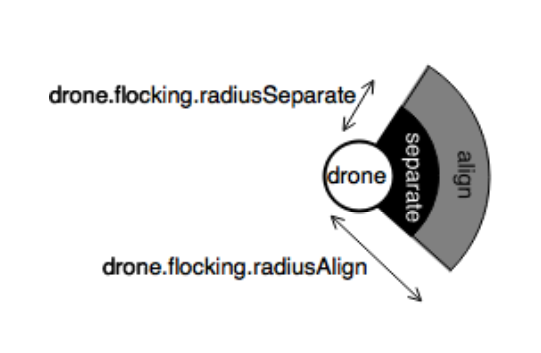
\includegraphics[width=0.4\paperwidth]{img/align.png}}
    \end{center}
    \caption{Area di riferimento per il comportamento \textit{Align}.}
    \label{align}
\end{figure}

\paragraph{Comportamento cohere:} il drone calcola il baricentro dei compagni di flock presenti nell'area di cohere, il cui raggio è \textbf{drone.flocking.radiusCohere}, e ruota in quella direzione.
La massima rotazione permessa è un angolo pari a \textbf{drone.flocking.maxCohereTurn}, più una quantità \textbf{drone.flocking.wiggleVar} casuale.

\begin{figure}[H] 
    \captionsetup{justification=centering, margin=2cm, font=footnotesize}
    \begin{center}
    \makebox[\textwidth]{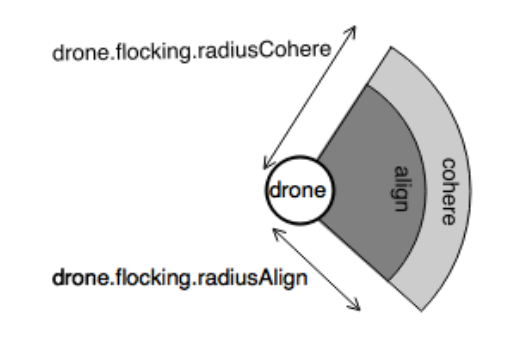
\includegraphics[width=0.4\paperwidth]{img/cohere.png}}
    \end{center}
    \caption{Area di riferimento per il comportamento \textit{Cohere}.}
    \label{cohere}
\end{figure}

\paragraph{Algoritmo di flocking:} come già ampiamente illustrato, il meccanismo di flocking è costituito da tre sottomeccanismi a priorità decrescente:
\begin{itemize}
    \item Separate;
    \item Align;
    \item Cohere.
\end{itemize}

Ad ogni ciclo di aggiornamento (\textit{tick}), può essere eseguito solo uno di questi comportamenti.
La figura \ref{activity_flocking} rappresenta il diagramma di attività dell'algoritmo di flocking, in cui viene omessa, per semplicità, la variabile casuale \textit{wiggleVar}.

\begin{figure}[H] 
    \captionsetup{justification=centering, margin=2cm, font=footnotesize}
    \begin{center}
    \makebox[\textwidth]{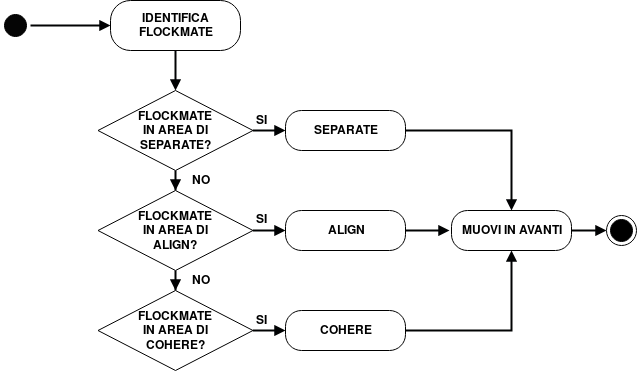
\includegraphics[width=0.5\paperwidth]{img/activity_flocking.png}}
    \end{center}
    \caption{Diagramma di attività dell'algoritmo di flocking.}
    \label{activity_flocking}
\end{figure}

Tutti i parametri di flocking sono fissati prima di avviare la simulazione ed influenzano il movimento del drone e dunque il comportamento del flock.

\begin{figure}[H] 
    \captionsetup{justification=centering, margin=2cm, font=footnotesize}
    \begin{center}
    \makebox[\textwidth]{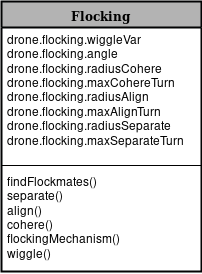
\includegraphics[width=0.2\paperwidth]{img/classe_flocking.png}}
    \end{center}
    \caption{Diagramma della classe Flocking.}
    \label{classe_flocking}
\end{figure}

\subsubsection{Progettazione del meccanismo di collision avoidance}

Il meccanismo di collision avoidance risulta indispensabile, considerato che i droni non devono scontrarsi tra loro o con gli ostacoli presenti all'interno dell'area simulata.
Tale meccanismo può essere suddiviso in due sottomeccanismi:

\begin{itemize}
    \item \textit{Obstacle avoidance}: permette di evitare collisioni tra un drone ed un ostacolo;
    \item \textit{Overlapping avoidance}: permette di evitare collisioni tra droni.
\end{itemize}

\paragraph{Modello di obstacle avoidance:} il modello segue una semplice regola: trovare il gap tra ostacoli che comporta la minima rotazione del drone verso il gap stesso. 
La semplicità di questa regola è dovuta al fatto che il drone ha un tempo limitato per riconoscere l’ostacolo, trovare il gap e ruotare verso la sua direzione.

In un contesto reale, il drone può trasportare un array di sensori ad infrarossi in grado di riconoscere le distanze e gli angoli degli ostacoli vicini. 
L’attività di riconoscimento di un ostacolo è modellata così come fatto per il sensing: un cono con un certo angolo e un certo raggio. 
Il drone, dopo aver calcolato le distanze e gli angoli degli ostacoli vicini, ricerca il gap che comporta la minore rotazione rispetto alla direzione corrente.

A causa della grande varietà di ostacoli che si possono trovare nei diversi contesti applicativi, sia la dimensione del gap che il raggio e l’angolo di visione degli ostacoli risultano configurabili. 
Durante la simulazione, questi parametri influenzano il comportamento del drone, perché l’algoritmo di obstacle avoidance dipende dal loro valore.

\begin{table}[H]
    \centering
    \resizebox{\textwidth}{!}{%
    \begin{tabular}{|l|l|c|}
    \hline
    \textbf{Parametro}             & \textbf{Definizione}                                                                                                                                               & \textbf{Unità di misura} \\ \hline
    drone.collision.gapAngle       &\begin{tabular}[c]{@{}l@{}}Minimo angolo che permette al drone di passare attraverso \\ il varco tra due ostacoli $\in$ (0, drone.sight.angleMax)\end{tabular}   & (gradi)                  \\ \hline
    drone.collision.vision         & Raggio di visibilità degli ostacoli                                                                                    & (m)                      \\ \hline
    drone.sight.angleMax           & Massimo angolo di visibilità degli ostacoli                                                                            & (gradi)                  \\ \hline
    \end{tabular}%
    }
    \caption{Parametri strutturali del meccanismo di obstacle avoidance.}
    \label{tabella_obstacle_avoidance}
\end{table}

Durante la simulazione, il drone esplora l'ambiente al fine di rilevare i target.
Per mantenere la sua operatività ed integrità, l'UAV deve evitare gli ostacoli.
Un'idea del funzionamento del meccanismo di obstacle avoidance è mostrato dalla figura \ref{obstacle_avoidance}.

\begin{figure}[H] 
    \captionsetup{justification=centering, margin=2cm, font=footnotesize}
    \begin{center}
    \makebox[\textwidth]{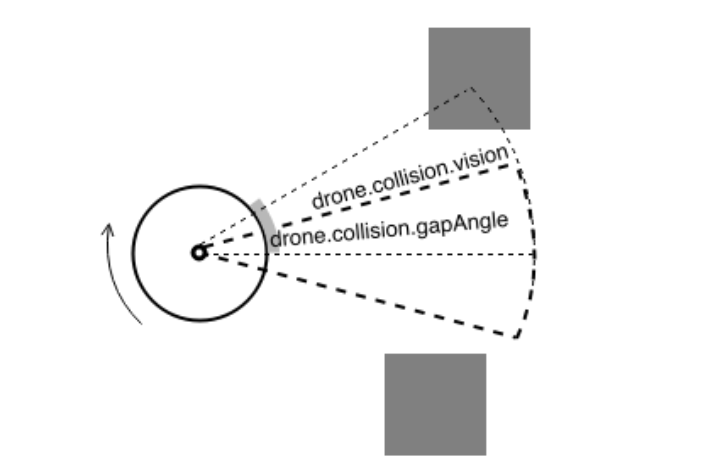
\includegraphics[width=0.4\paperwidth]{img/obstacle_avoidance.png}}
    \end{center}
    \caption{Principio di funzionamento del meccanismo di obstacle avoidance.}
    \label{obstacle_avoidance}
\end{figure}

L’algoritmo opera nel seguente modo:
\begin{itemize}
	\item Prima di controllare la presenza di ostacoli, il drone deve verificare se è rimasto fermo sulla stessa posizione per un certo numero di ticks consecutivi.
	\item Se risulta bloccato, significa che l’ostacolo presente di fronte al drone è probabilmente un muro che gli impedisce di avanzare. 
    Al fine di evitare lo stallo, il drone esegue un movimento rotazionale di 90$^{\circ}$ più una quantità casuale \textbf{drone.flocking.wiggleVar}.
	\item Viceversa, se il drone non è bloccato, allora controlla la presenza di ostacoli.
	\item Se non ci sono ostacoli, significa che il drone può avanzare senza alcun problema.
	\item Se sono rilevati degli ostacoli, il drone controlla la presenza del varco tra essi, in riferimento ad un certo angolo di gap.
	\item Se il varco non viene trovato, allora il drone ruota leggermente in direzione oraria o antioraria (la direzione viene scelta casualmente), al fine di ricercare un altro gap vicino. 
    Questo angolo di rotazione è pari alla metà di \textbf{drone.sight.angleMax}. 
    Successivamente, il drone effettua una decelerazione, perché si trova di fronte a ostacoli senza varco.
	\item Se il varco viene trovato, allora il drone esegue una rotazione verso il gap. 
    Anche in questo caso il drone decelera, perché il varco potrebbe essere stretto e dunque il drone deve attraversarlo con attenzione.
\end {itemize}

\begin{figure}[H] 
    \captionsetup{justification=centering, margin=2cm, font=footnotesize}
    \begin{center}
    \makebox[\textwidth]{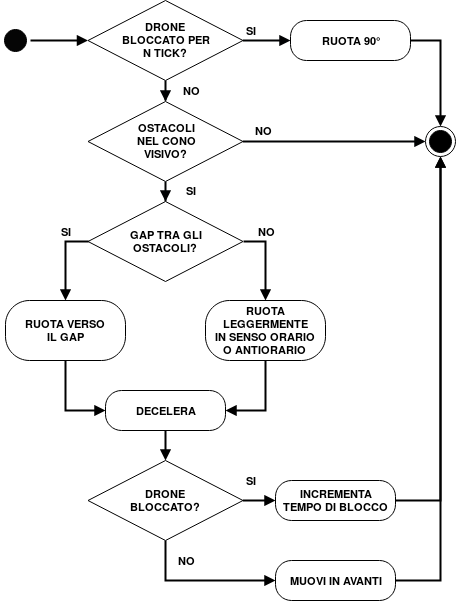
\includegraphics[width=0.4\paperwidth]{img/activity_obstacle.png}}
    \end{center}
    \caption{Diagramma di attività del meccanismo di obstacle avoidance.}
    \label{activity_obstacle}
\end{figure}

La figura \ref{classe_obstacle} illustra il diagramma di classe relativo al meccanismo di obstacle avoidance.
Gli attributi \textbf{drone.collision.gapAngle}, \textbf{drone.collision.vision} e \textbf{drone.sight.angleMax} sono configurati prima dell'avvio della simulazione, mentre i restanti due vengono utilizzati per contare il numero di collisioni e l'eventuale tempo di blocco di un drone su una patch.

\begin{figure}[H] 
    \captionsetup{justification=centering, margin=2cm, font=footnotesize}
    \begin{center}
    \makebox[\textwidth]{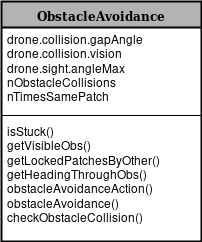
\includegraphics[width=0.2\paperwidth]{img/classe_obstacle.png}}
    \end{center}
    \caption{Diagramma della classe ObstacleAvoidance.}
    \label{classe_obstacle}
\end{figure}

\paragraph{Modello di overlapping avoidance:} il solo meccanismo di obstacle avoidance non è sufficiente per evitare le sovrapposizioni tra i droni, perché un drone non può prevedere i movimenti degli altri droni. 
Al fine di evitare questo tipo di problema, si è progettato un modello di overlapping avoidance tra droni: conoscendo l’accelerazione, la decelerazione, la velocità massima e la rotazione massima di un drone nell’arco di una finestra temporale, si può calcolare la regione di raggiungibilità (\textit{reachable region}), ovvero la regione che, in termini di patch, il drone potrebbe ricoprire nei prossimi ticks. 

In particolare, la strategia per evitare le sovrapposizioni tra i droni prevede, in primo luogo, di schedulare una regione conica di raggiungibilità e, in secondo luogo, di trattare le regioni già schedulate dagli altri droni come ostacoli, applicando il meccanismo di obstacle avoidance. 
In questo modo, le potenziali regioni in cui un drone può trovarsi nell’immediato futuro non sono accessibili dagli altri droni. 

Il meccanismo di overlapping avoidance dei droni risulta altresì configurabile: il numero di droni può variare notevolmente tra i diversi scenari applicativi e le caratteristiche tecniche come velocità massima e massima rotazione risultano molto diverse tra modelli di drone differenti. 
La regione conica schedulata da un drone per evitare le collisioni è descritta da un certo raggio ed un certo angolo, come riportato nella seguente tabella.

\begin{table}[H]
    \centering
    \begin{tabular}{|l|l|c|}
    \hline
    \textbf{Parametro}              & \textbf{Definizione}                      & \textbf{Unità di misura}      \\ \hline
    drone.reachable.radius          & Angolo delle patch schedulate             & (gradi)                       \\ \hline
    drone.reachable.angle           & Raggio delle patch schedulate             & (m)                           \\ \hline
    \end{tabular}%
    \caption{Parametri strutturali del meccanismo di overlapping avoidance.}
    \label{tabella_obstacle_avoidance}
\end{table}

L'algoritmo di overlapping avoidance tra UAV, come si evince dalla suddetta descrizione, è suddiviso in due fasi:

\begin{enumerate}
    \item \textit{Scheduling delle celle};
    \item \textit{Azione di overlapping avoidance}.
\end{enumerate}

Di seguito vengono illustrate tutte le casistiche della fase di prenotazione delle patch:

\begin{enumerate} [label=(\alph*)]
    \item Nel caso generale, il drone identifica le patch libere sotto la sua posizione ed all'interno del cono di raggiungibilità e le blocca.
    \begin{figure}[H] 
        \captionsetup{justification=centering, margin=2cm, font=footnotesize}
        \begin{center}
        \makebox[\textwidth]{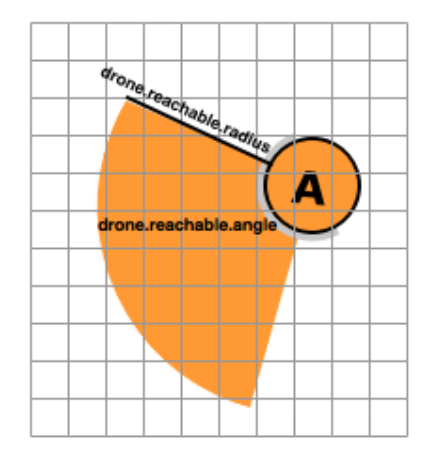
\includegraphics[width=0.2\paperwidth]{img/overlapping_a.png}}
        \end{center}
        \caption{Caso generale: prenotazione delle patch nella regione di raggiungibilità.}
        \label{overlapping_a}
    \end{figure}
    \item In altri casi, le regioni di scheduling possono risultare sovrapposte.
    Nella figura \ref{overlapping_b} l'UAV A blocca le celle nel cono arancione.
    L'UAV B, di conseguenza, identifica le celle già bloccate da A e prenota solo le patch disponibili in quel preciso istante, ovvero le celle presenti nel cono blu.
    \begin{figure}[H] 
        \captionsetup{justification=centering, margin=2cm, font=footnotesize}
        \begin{center}
        \makebox[\textwidth]{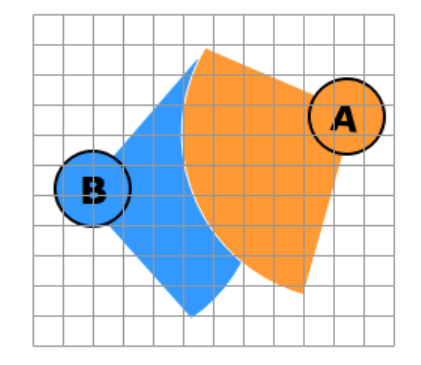
\includegraphics[width=0.2\paperwidth]{img/overlapping_b.png}}
        \end{center}
        \caption{Caso di sovrapposizione dello scheduling delle patch.}
        \label{overlapping_b}
    \end{figure}
    \item I casi (a) e (b) potrebbero portare ad un problema di \textit{deadlock}, nell'eventualità in cui un drone A, che si trova esattamente dietro il drone B, prenota le patch davanti a B.
    In questo caso il drone B non può avanzare, in quanto tutte le celle raggiungibili sono già prenotate.
    \begin{figure}[H] 
        \captionsetup{justification=centering, margin=2cm, font=footnotesize}
        \begin{center}
        \makebox[\textwidth]{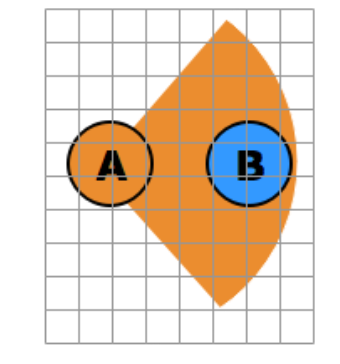
\includegraphics[width=0.2\paperwidth]{img/overlapping_c.png}}
        \end{center}
        \caption{Caso di deadlock.}
        \label{overlapping_c}
    \end{figure}
    Al fine di evitare tale situazione, risulta necessario introdurre un ulteriore requisito: un drone, prima di eseguire la prenotazione delle celle, deve controllare se all'interno del cono di scheduling è presente un altro UAV.
    Se il controllo ha esito positivo (è presente un drone nel cono), verrà schedulata solo la cella sottostante il drone che ha effettuato il controllo.
\end{enumerate}

Il diagramma di attività che descrive l'algoritmo di scheduling è mostrato in figura \ref{activity_scheduling}.

\begin{figure}[H] 
    \captionsetup{justification=centering, margin=2cm, font=footnotesize}
    \begin{center}
    \makebox[\textwidth]{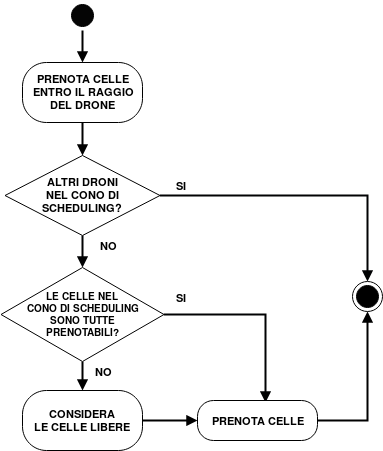
\includegraphics[width=0.3\paperwidth]{img/activity_scheduling.png}}
    \end{center}
    \caption{Diagramma di attività del meccanismo di obstacle avoidance.}
    \label{activity_scheduling}
\end{figure}

Di seguito, invece, è possibile osservare il diagramma della classe DronesOverlapAvoidance: gli attributi relativi al raggio ed all'angolo del cono di scheduling devono essere configurati prima dell'esecuzione del simulatore e dipendono dalla velocità di crociera assunta dal drone.
I rimanenti parametri variano durante la simulazione.

\begin{figure}[H] 
    \captionsetup{justification=centering, margin=2cm, font=footnotesize}
    \begin{center}
    \makebox[\textwidth]{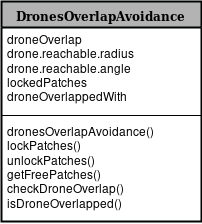
\includegraphics[width=0.2\paperwidth]{img/classe_overlapping.png}}
    \end{center}
    \caption{Diagramma della classe ObstacleAvoidance.}
    \label{classe_overlapping}
\end{figure}

\subsubsection{Progettazione dell'impronta di feromone attrattivo}

Un drone rilascia un’impronta di feromone attrattivo quando rileva un target, al fine di “richiamare” altri droni attivando il meccanismo di coordinamento basato su stigmergia. 

Un’impronta di feromone è modellata come un tronco di cono e tipicamente ricopre più celle dello spazio di ricerca. 
Più impronte di feromone rilasciate in prossimità spazio-temporale si aggregano a formare una traccia feromonica che evapora nel tempo. 

L’impronta è caratterizzata da un raggio centrale (\textbf{mark.RadiusTop}), da un raggio periferico (\textbf{mark.radiusDown}) e da un tasso di diffusione (\textbf{track.diffRate}), mentre la traccia feromonica è caratterizzata da un tasso di evaporazione superficiale (\textbf{track.evapRate}). 

Le funzioni eseguite sulla traccia feromonica sono:
\begin{itemize}
	\item \textit{Evaporazione};
	\item \textit{Diffusione} (opzionale).
\end{itemize}

\paragraph{Impronta e traccia feromonica:} di seguito viene illustrato il modello dell'impronta e della traccia di feromone attrattivo, insieme ai parametri caratteristici.

\begin{figure}[H] 
    \captionsetup{justification=centering, margin=2cm, font=footnotesize}
    \begin{center}
    \makebox[\textwidth]{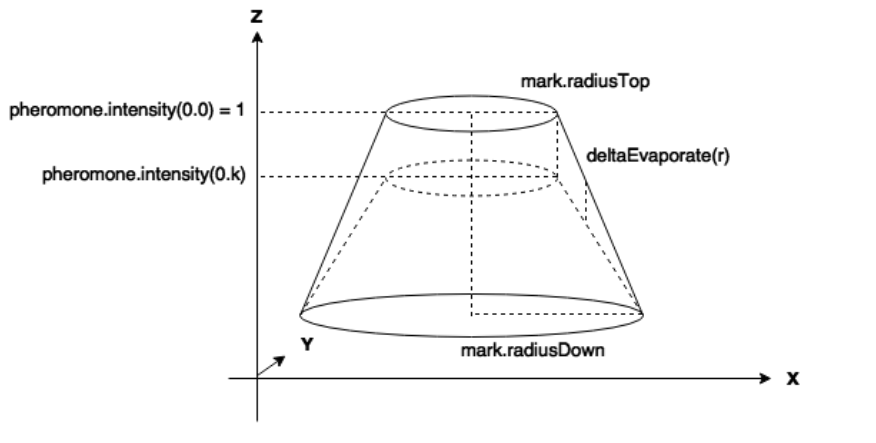
\includegraphics[width=0.4\paperwidth]{img/modello3d_feromone.png}}
    \end{center}
    \caption{Modello tridimensionale dell'impronta di feromone attrattivo.}
    \label{modello3d_feromone}
\end{figure}

\begin{figure}[H] 
    \captionsetup{justification=centering, margin=2cm, font=footnotesize}
    \begin{center}
    \makebox[\textwidth]{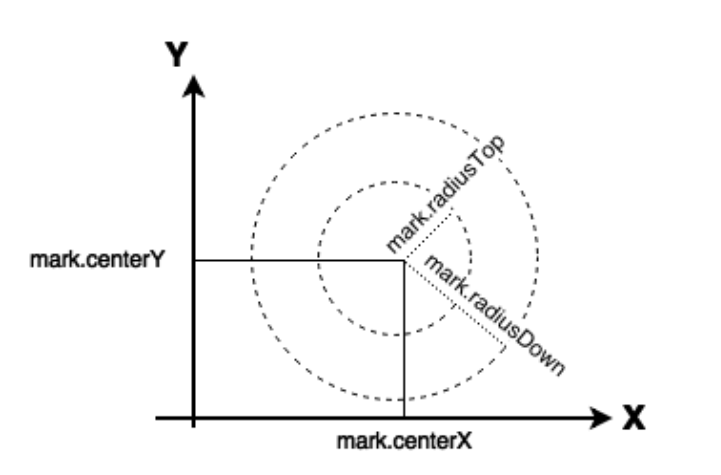
\includegraphics[width=0.4\paperwidth]{img/modello2d_feromone.png}}
    \end{center}
    \caption{Modello bidimensionale dell'impronta di feromone attrattivo.}
    \label{modello2d_feromone}
\end{figure}

\begin{table}[H]
    \centering
    \resizebox{\textwidth}{!}{%
    \begin{tabular}{|l|l|c|}
    \hline
    \textbf{Parametro}              & \textbf{Definizione}                                                                                  & \textbf{Unità di misura}      \\ \hline
    mark.centerX                    & Coordinata X del centro di rilascio dell'impronta di feromone                                         & (-)                           \\ \hline
    mark.centerY                    & Coordinata Y del centro di rilascio dell'impronta di feromone                                         & (-)                           \\ \hline
    mark.radiusTop                  & Raggio di rilascio iniziale dell'impronta di feromone $\in$ [0, +$\infty$)                            & (m)                           \\ \hline
    mark.radiusDown                 & Raggio di rilascio diffuso iniziale dell'impronta di feromone $\in$ [mark.radiusTop, +$\infty$)       & (m)                           \\ \hline
    track.evapRate                  & Tasso di evaporazione della traccia di feromone $\in$ [0,1]                                           & (adimensionale)               \\ \hline
    \end{tabular}%
    }
    \caption{Parametri strutturali dell'impronta di feromone.}
    \label{tabella_feromone}
\end{table}

L'intensità di rilascio dell'impronta di feromone attrattivo al tick 0 è pari a:

\begin{equation*}
    pheromone.intensity (r,0) = 1 \; , \; r < mark.radiusTop
\end{equation*}

L'intensità decresce a partire da \textbf{mark.radiusTop} fino a \textbf{mark.radiusDown} in accordo alla seguente espressione:

\begin{equation*}
    \resizebox{\textwidth}{!} 
    {
        $ pheromone.intensity (r,k) = pheromone.intensity (0,k) \cdot \frac{r - mark.radiusDown}{mark.radiusTop - mark.radiusDown} $
    }
\end{equation*}

dove

\begin{equation*}
    mark.radiusTop < r < mark.radiusDown , \; k \ge 0
\end{equation*}

\begin{figure}[H] 
    \captionsetup{justification=centering, margin=2cm, font=footnotesize}
    \begin{center}
    \makebox[\textwidth]{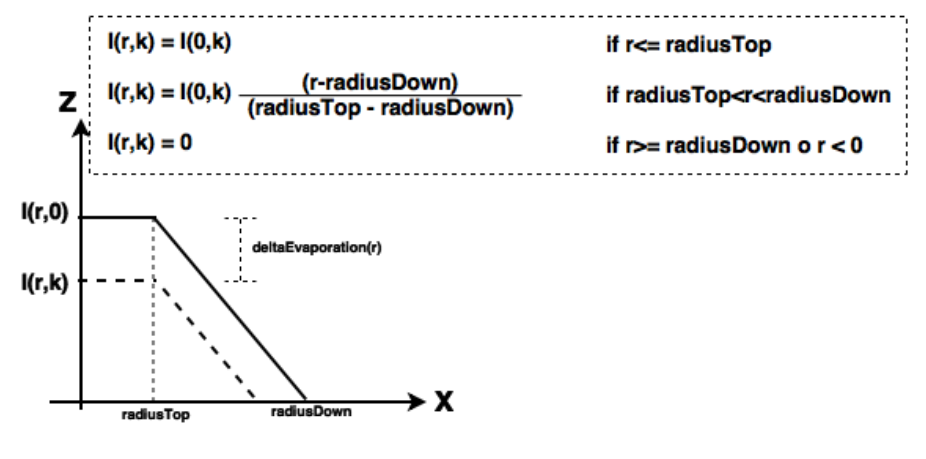
\includegraphics[width=0.5\paperwidth]{img/evaporazione.png}}
    \end{center}
    \caption{Modello dell'intensità di feromone e comportamento di evaporazione.}
    \label{evaporazione}
\end{figure}

\paragraph{Comportamento di evaporazione:} l’evaporazione rappresenta il decadimento lineare della traccia di feromone nel tempo. 
Ad ogni ciclo di aggiornamento il feromone evapora di una certa quantità a partire da quando viene rilasciato e dopo un certo tempo, a seconda del valore del tasso di evaporazione, il feromone scompare completamente. 

Dal momento che il tempo simulato è discretizzato e l’evaporazione è lineare, ad ogni ciclo di aggiornamento viene sottratta da ogni patch sempre la stessa quantità di feromone. 
Ad esempio, se il tasso di evaporazione è pari a 0.1, dopo 10 ticks, il feromone scompare completamente indipendentemente dalla sua intensità iniziale. 

L’espressione matematica che descrive l’evaporazione feromonica è la seguente:
\begin{equation*}
    pheromone.intensity(r,k) = pheromone.intensity(r,k-1) \; - \; deltaEvaporation(r)
\end{equation*}

dove
\begin{itemize}
    \item $deltaEvaporation(r) = evapRate \cdot pheromone.intensity(r,0)$, ovvero la quantità di feromone che evapora ad ogni tick;
    \item $pheromone.intensity(r,k)$ rappresenta l'intensità dell'impronta feromonica in funzione della distanza r dal centro di rilascio e del numero di tick k;
    \item $pheromone.intensity(r,0)$ rappresenta l'intensità dell'impronta feromonica al momento del rilascio in funzione della distanza r dal centro di rilascio.
\end{itemize}

\paragraph{Meccanismo di coordinamento basato su stigmergia:} come già evidenziato in precedenza, la stigmergia è un meccanismo emergente.
Il meccanismo di coordinamento basato su stigmergia segue due semplici regole:
\begin{itemize}
	\item se un drone rileva un target, vi rilascia sopra un’impronta feromonica;
	\item se un drone rileva un’impronta feromonica, segue la direzione corrispondente al picco di intensità. 
\end{itemize}

Tale meccanismo ha la potenzialità di attrarre gruppi di droni che sono posizionati in prossimità spazio-temporale rispetto alla traccia feromonica. 

\paragraph{Assuefazione olfattiva:} un altro importante meccanismo da evidenziare è rappresentato dall’assuefazione olfattiva (\textit{olfactory habituation}). 
Un’agente, dopo aver rilevato del feromone per un certo numero di ticks, ne diventa assuefatto, ovvero non è più in grado di percepirne la presenza e, di conseguenza, non ne viene influenzato. 

L’assuefazione olfattiva risulta importante per due ragioni:
\begin{itemize}
    \item evita di attrarre un numero eccessivo di agenti sullo stesso target;
	\item evita di rimanere nei pressi dello stesso target per troppo tempo.
\end{itemize}

Questi due aspetti permettono di ridurre la probabilità di collisioni ed il tempo impiegato nella ricerca di target in prossimità spaziale. 

L’assuefazione olfattiva è caratterizzata da un parametro che esprime la quantità di tempo entro la quale un drone deve annusare il feromone prima di ignorarlo. 
Questo è un parametro configurabile in modo da poter essere modificato in funzione dello specifico contesto applicativo. 

Il seguente diagramma di attività illustra il meccanismo di funzionamento dell’assuefazione olfattiva.

\begin{figure}[H] 
    \captionsetup{justification=centering, margin=2cm, font=footnotesize}
    \begin{center}
    \makebox[\textwidth]{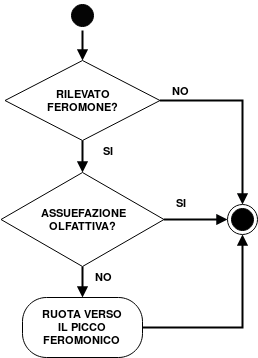
\includegraphics[width=0.2\paperwidth]{img/activity_assuefazione.png}}
    \end{center}
    \caption{Diagramma di attività relativo al funzionamento dell'assuefazione olfattiva.}
    \label{activity_assuefazione}
\end{figure}

Di seguito, invece, sono evidenziati tutti gli attributi ed i metodi relativi al feromone attrattivo.
Tali attributi, eccetto \textbf{mark.deltaEvaporate}, devono essere configurati prima dell'inizio della simulazione.

\begin{figure}[H] 
    \captionsetup{justification=centering, margin=2cm, font=footnotesize}
    \begin{center}
    \makebox[\textwidth]{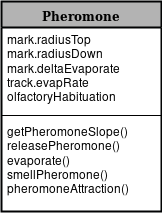
\includegraphics[width=0.2\paperwidth]{img/classe_pheromone.png}}
    \end{center}
    \caption{Diagramma della classe Pheromone.}
    \label{classe_pheromone}
\end{figure}

\subsubsection{Progettazione del meccanismo di rilevamento ed esecuzione dei target}

Come già evidenziato nella fase di analisi, il drone è equipaggiato con uno o più sensori. 
Si suppone che un sensore sia ideale e la sua copertura sia modellata attraverso un cono di sensing, con un angolo e un raggio definiti a priori.

Durante l’esplorazione, possiamo avere tre diversi casi, in relazione al rilevamento dei target:
\begin {itemize}
	\item Nessun target rilevato: il drone prosegue normalmente la sua esplorazione;
	\item Un solo target rilevato: il drone rilascia un’impronta feromonica centrata sulle coordinate dell’obiettivo;
	\item Più target rilevati: invece di rilasciare più impronte di feromone, il drone ne rilascia un sola in corrispondenza del target più vicino, come evidenziato nella figura \ref{rilevamento_multiplo_target}.
	In questo modo, il drone rilascerà le impronte feromoniche sugli altri target nei tick immediatamente successivi.
\end{itemize}

\begin{figure}[H] 
    \captionsetup{justification=centering, margin=2cm, font=footnotesize}
    \begin{center}
    \makebox[\textwidth]{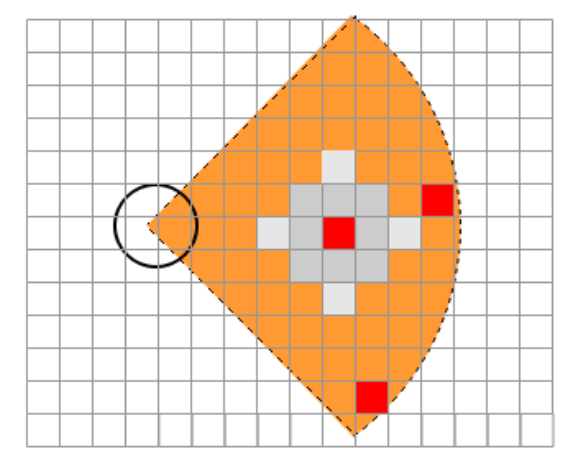
\includegraphics[width=0.4\paperwidth]{img/rilevamento_multiplo_target.png}}
    \end{center}
    \caption{Meccanismo di rilascio del feromone in caso di rilevamento multiplo di target.}
    \label{rilevamento_multiplo_target}
\end{figure}



\subsection{Algortmi PAPER}

Nella fase di analisi abbiamo introdotto la strategia adottata dagli autori di \cite{palmieri2017comparison}, i quali hanno applicato tre diversi algoritmi bio-ispirati per investigare i comportamenti emergenti di uno sciame di robot.
La missione di questi agenti consiste nel rilevare dei target distribuiti in maniera uniforme in un'area limitata, attraverso delle metaeuristiche di esplorazione e reclutamento.
All'interno del modulo responsabile di ospitare gli algoritmi integrati per un'analisi comparativa, in ogni caso, gli attori non sono dei robot ma nuovamente dei droni, che mantengono molte delle caratteristiche analizzate nelle sezioni precedenti.

Per una migliore comprensione dell'argomento passeremo prima in rassegna i punti chiave dell'algoritmo di esplorazione e successivamente ci concentreremo sugli algoritmi di reclutamento precedentemente introdotti.

\subsubsection{Strategia di esplorazione}

L'obiettivo dei droni, in questa prima fase, è quello di rilevare i target distribuiti nell'ambiente.
Per ottimizzare la ricerca di questi obiettivi, gli autori hanno introdotto un meccanismo stigmergico legato ad un feromone repulsivo.
In questo modo, un drone che deve selezionare la cella successiva analizza prima il subset di patch ad esso vicine (o \textit{neighborhood}) e, successivamente, seleziona la cella che presenta la traccia feromonica di minore intensità.

\paragraph{Diffusione del feromone:} il feromone viene depositato dal drone non appena si muove in una nuova posizione.
La struttura del feromone prevede la diffusione dello stesso entro un raggio $R_S$.
Ogni cella ha un livello feromonico iniziale uguale a 0, a voler rappresentare che la patch non è stata mai visitata.

Ipotizziamo che un drone $k$, all'istante $t$, si trova nella cella di coordinate ($x_k$,$y_k$).
La quantità di feromone depositata sulle celle di coordinata ($x$,$y$), all'interno dell'area descritta dal raggio $R_S$, è data da:

\begin{equation}
    \Delta\tau_{c}^{k,t} = 
    \begin{cases}
        \Delta\tau_{0}e^{\frac{-r_{kc}}{a_1}} - \frac{\epsilon}{a_2} &\text{per $r_{kc} \leq R_S$}\\
        0 &\text{altrimenti}
    \end{cases}
\end{equation}
Dove:
\begin{itemize}
    \item $r_{kc}$ è la distanza tra il drone $k$ e la cella $c$ ed è definita come:
    \begin{equation}
        r_{kc} = \sqrt{(x^{t}_{k} - x)^{2} + (y^{t}_{k} - y)^{2}}
    \end{equation}
    \item $\Delta\tau_{0}$ rappresenta la quantità iniziale di feromone che un agente rilascia sulla cella su cui è posizionato;
    \item $\epsilon \in (0,1)$ è una variabile euristica atta a modellare il rumore;
    \item $a_{1}$ e $a_{2}$ sono costanti utilizzate per ridurre o aumentare gli effetti di feromone e rumore, rispettivamente. 
\end{itemize} 

Più droni possono depositare feromone sulla stessa patch.
La quantità totale di feromone all'interno di una cella sarà data dalla somma algebrica delle quantità depositate dai vari agenti.

\'E previsto un meccanismo di evaporazione della traccia feromonica che dipende da un parametro configurabile, detto \textit{tasso di evaporazione} $\rho$.
La quantità di feromone evaporata in una generica cella \textit{c}, all'istante \textit{t}, è data da:
\begin{equation}
    \xi_{t}^{c} = \rho \cdot \tau_{c}^{t}
\end{equation}
Dove $\tau_{c}^{t}$ è la quantità totale di feromone depositata sulla cella \textit{c} all'istante \textit{t}.

Per il calcolo di $\rho$ viene utilizzato il coefficiente $ERTU_{\%}$ (Evaporation Rate Time Unit), che riguarda il tasso di evaporazione per unità di tempo.
Siano $t_{v}$ l'istante corrispondente all'ultima visita in una cella e $t$ l'istante corrente.
$(t - t_{v})$ è dunque il tempo trascorso dall'ultima visita. 
La percentuale di feromone evaporato nell'intervallo di tempo preso in esame è dato da:
\begin{equation}
    \rho = (t - t_{v}) \cdot ERTU_{\%}
\end{equation}

Considerando l'evaporazione del feromone e la diffusione in accordo con la distanza dalla cella di rilascio, la quantità totale di feromone in una generica cella \textit{c}, all'iterazione \textit{t}, è data dall'espressione:
\begin{equation}\label{rule18}
    \tau_{c}^{t} = \tau_{c}^{t-1} - \xi_{c}^{t} + \sum_{k=1}^{N^{D}} \Delta\tau_{c}^{k,t}
\end{equation}
Dove $N^{D}$ è il numero totale di droni che hanno depositato il feromone.

Nella figura \ref{diffusione_feromone} è possibile osservare un esempio di diffusione feromonica.

\begin{figure}[H] 
    \captionsetup{justification=centering, margin=2cm, font=footnotesize}
    \begin{center}
    \makebox[\textwidth]{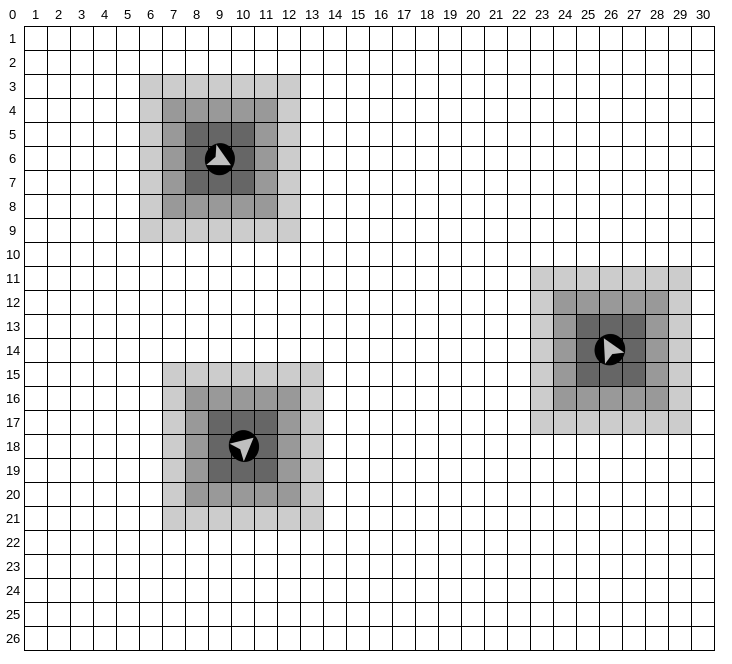
\includegraphics[width=0.4\paperwidth]{img/diffusione_feromone.png}}
    \end{center}
    \caption{Esempio di diffusione del feromone.}
    \label{diffusione_feromone}
\end{figure}

\paragraph{Selezione cella successiva:} ciascun drone $k$, ad ogni iterazione $t$, è posizionato in una particolare patch $c_{k}^{t}$, circondata dal set $N(c_{k}^{t})$ di celle accessibili da quella posizione, denominato \textit{neighborhood}.

Ogni drone rileva il feromone depositato in $N(c_{k}^{t})$ e, successivamente, seleziona la cella in cui muoversi all'iterazione successiva.

La probabilità, all'istante $t$, che un agente $k$ ha di muoversi dalla cella $c_{k}^{t}$ ad una $c \in N(c_{k}^{t})$ può essere calcolata attraverso la seguente relazione:
\begin{equation}\label{rule19}
    p(c|c_{k}^{t}) = \frac{(\tau_{c}^{t})^{\phi} \cdot (\eta_{c}^{t})^{\lambda}}{\sum_{b \in N(c_{k}^{t})}(\tau_{b}^{t})^{\phi} \cdot (\eta_{b}^{t})^{\lambda}} \; , \; \forall c \in N(c_{k}^{t})
\end{equation}
Dove:
\begin{itemize}
    \item $(\tau_{c}^{t})^{\phi}$ rappresenta la quantità di feromone nella cella $c$ al tick $t$;
    \item $(\eta_{c}^{t})^{\lambda}$ è una variabile euristica, necessaria ad evitare che un drone resti intrappolato in un minimo locale;
    \item $\phi$ e $\lambda$ sono due costanti parametriche, utilizzate per bilanciare i pesi dati al feromone ed alla variabile euristica, rispettivamente.
\end{itemize}
Il drone $k$ selezionerà, dunque, la patch che soddisfa la seguente condizione:
\begin{equation}
    c = min[p(c|c_{k}^{t})]\label{rule20}
\end{equation}
In questo modo, l'agente si dirigerà verso zone inesplorate, ottimizzando l'esplorazione dell'area ed il rilevamento dei target non ancora trovati.

\paragraph{Algoritmo di esplorazione:} questo algoritmo è un processo iterativo. 
Alla prima iterazione, ogni cella ha lo stesso valore di intensità feromonica, in modo da rendere quasi casuale la selezione di una patch.
Alle iterazioni successive, i droni si muovono da una cella all'altra secondo le regole espresse in \ref{rule19} e \ref{rule20}.
La traccia di feromone sulle celle visitate è aggiornata secondo \ref{rule18}, così da aumentare la probabilità che le celle con intensità feromonica nulla vengano visitate.

L'obiettivo è quello di ridurre comportamenti di sovrapposizione o ridondanza, in modo da rendere ancor più efficente il completamento della missione.

L'algoritmo termina l'esecuzione nel momento in cui il drone diventa \textit{coordinator} o \textit{recruited}, come vedremo più avanti, oppure se la missione è completa.

\begin{figure}[H] 
    \captionsetup{justification=centering, margin=2cm, font=footnotesize}
    \begin{center}
    \makebox[\textwidth]{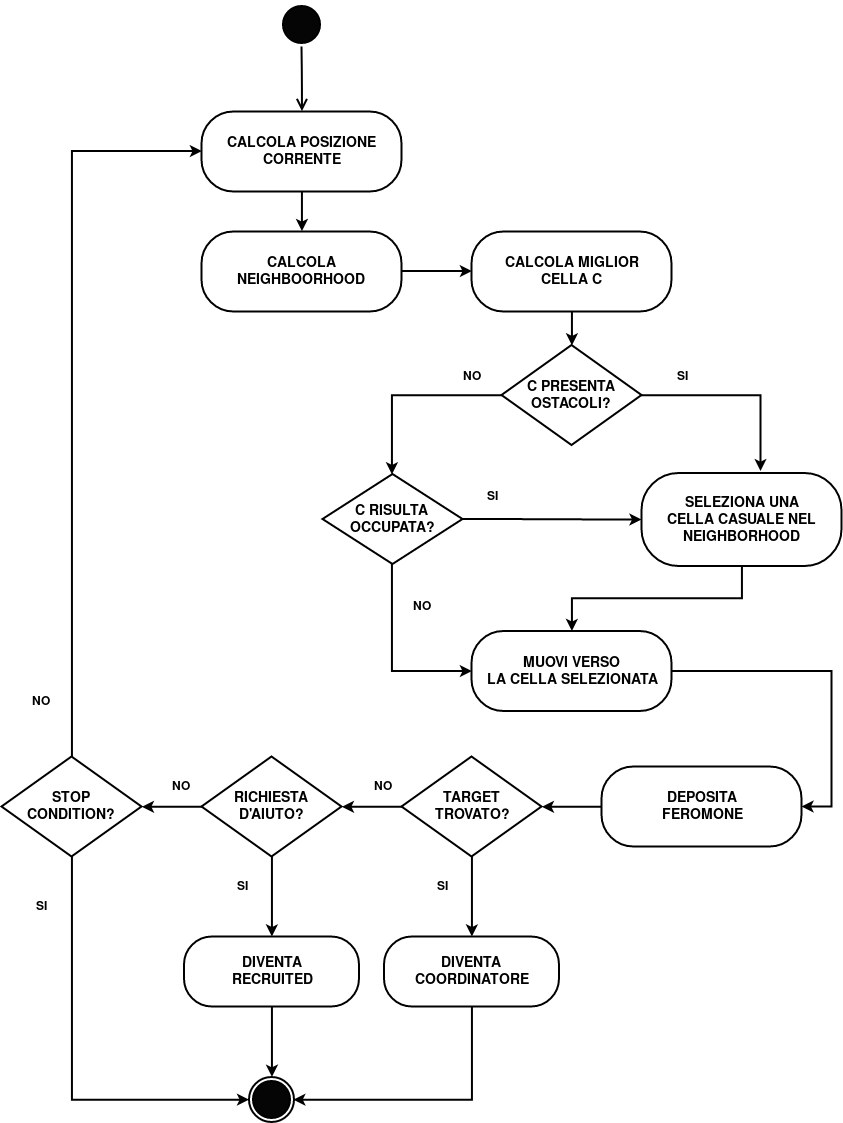
\includegraphics[width=0.5\paperwidth]{img/attivita_exploration.png}}
    \end{center}
    \caption{Diagramma di attività per la strategia di esplorazione.}
    \label{attivita_exploration}
\end{figure}

\subsubsection{Strategie di reclutamento}

Quando un drone identifica un target, esso diventa \textit{coordinator} ed inizia una procedura di reclutamento di altri agenti, per poter lavorare l'obiettivo in modo cooperativo.
Tale procedura prevede l'utilizzo di una comunicazione wireless per rintracciare i droni che risultano posizionati entro un raggio $R_t$.
I pacchetti inviati contengono le coordinate del mittente che, non appena lette da un drone in stato d'esplorazione, portano quest'ultimo a cambiare il proprio stato in \textit{recruited} ed a raggiungere il coordinatore.

Come accennato nella sezione \ref{elemento_target}, è necessario che un numero minimo di droni raggiunga il target, prima che questi possa essere lavorato e che la comunicazione del coordinatore venga interrotta.

Di seguito illustriamo tre differenti metaeuristiche per le gestione della fase di reclutamento.

\paragraph{Strategia di reclutamento FTS-RR:} l'algoritmo \textit{Firefly-based team strategy for robots recruitment} è una strategia di ispirazione biologica, basato sul comportamento delle lucciole.

In particolare, quando un drone identifica un target, questo diventa \textit{coordinatore} ed inizia ad attrarre gli altri droni come una lucciola.

Gli elementi più importanti sono la \textit{variazione di intensità luminosa} ed il cosiddetto \textit{coefficiente di attrattività}.
Il primo fattore dipende dalla distanza tra due lucciole, il secondo è funzione del primo e, di conseguenza, anche della distanza.

La distanza tra due lucciole $i$ e $j$, posizionate rispettivamente in ($x_i,y_i$) e ($x_j,y_j$), può essere definita come la distanza Euclidea, data da:
\begin{equation}
    r_{ij} = \sqrt{(x_i - x_j)^2 \; + \; (y_i - y_j)^2}
\end{equation}

Poiché la funzione di attrattività di una lucciola varia in base a $r_{ij}$, si può selezionare una qualunque funzione monotona decrescente dipendente dalla distanza tra le due lucciole.
Possiamo dunque utilizzare la seguente funzione esponenziale:
\begin{equation}\label{rule23}
    \beta = \beta_{0} e^{- \gamma r_{ij}^{2}}
\end{equation}
Dove:
\begin{itemize}
    \item $\beta_{0}$ rappresenta l'attrattività iniziale a distanza $r_{ij} = 0$;
    \item $\gamma$ è il coefficiente di assorbimento alla fonte che regola la diminuzione di intensità luminosa.
\end{itemize}

Il movimento di una lucciola $i$, che è attratta da una lucciola più luminosa $j$, nella sequenza di tick $t \rightarrow t+1$, è regolato dalle seguenti relazioni:
\begin{equation}\label{rule25}
    \begin{cases}
        x_{i}^{t+1} = x_{i}^{t} + \beta_{0} e^{- \gamma r_{ij}^{2}} (x_{j}^{t} - x_{i}^{t}) + \alpha(\sigma - \frac{1}{2}) \\
        y_{i}^{t+1} = y_{i}^{t} + \beta_{0} e^{- \gamma r_{ij}^{2}} (y_{j}^{t} - y_{i}^{t}) + \alpha(\sigma - \frac{1}{2})
    \end{cases}    
\end{equation}

Dove:
\begin{itemize}
    \item $x_{i}^{t}$ e $y_{i}^{t}$ rappresentano le coordinate della posizione corrente;
    \item $\beta_{0} e^{- \gamma r_{ij}^{2}} (x_{j}^{t} - x_{i}^{t})$ e $\beta_{0} e^{- \gamma r_{ij}^{2}} (y_{j}^{t} - y_{i}^{t})$ sono utilizzati per modellare l'attrattiva della lucciola $i$ come l'intensità della luce vista dalle lucciole adiacenti;
    \item $\alpha(\sigma - \frac{1}{2})$ è un termine di randomizzazione, con $\alpha$ parametro di randomizzazione che dipende dalla missione;
    \item $\sigma$ rappresenta il fattore che regola la distanza di visibilità ed in molti casi può essere settato a 1.
\end{itemize}

Prendiamo adesso in esame il caso in cui un drone riceve più di una richiesta d'aiuto: in questo caso si muoverà verso il target più luminoso, secondo la relazione \ref{rule23}.
Il movimento di un drone è dunque condizionato sia dalla distanza con il target che da una componente randomica, atta ad evitare che l'agente rimanga incastrato in un minimo locale.

Affinché le relazioni in \ref{rule25} possano essere applicabili ad un contesto discreto, come nel caso dell'ambiente di simulazione, gli autori hanno trovato necessario modificarle come segue.
Per la coordinata $x$:
\begin{equation}
    \begin{cases}
        x_{i}^{t+1} = x_{i}^{t} + 1 , \text{se}[\beta_{0} e^{- \gamma r_{ij}^{2}} (x_{j}^{t} - x_{i}^{t}) + \alpha(\sigma - \frac{1}{2}) > 0]\\
        x_{i}^{t+1} = x_{i}^{t} - 1 , \text{se}[\beta_{0} e^{- \gamma r_{ij}^{2}} (x_{j}^{t} - x_{i}^{t}) + \alpha(\sigma - \frac{1}{2}) < 0]\\
        x_{i}^{t+1} = x_{i}^{t} , \text{se}[\beta_{0} e^{- \gamma r_{ij}^{2}} (x_{j}^{t} - x_{i}^{t}) + \alpha(\sigma - \frac{1}{2}) = 0]
    \end{cases}
\end{equation}
Mentre per la coordinata $y$:
\begin{equation}
    \begin{cases}
        y_{i}^{t+1} = y_{i}^{t} + 1 , \text{se}[\beta_{0} e^{- \gamma r_{ij}^{2}} (y_{j}^{t} - y_{i}^{t}) + \alpha(\sigma - \frac{1}{2}) > 0]\\
        y_{i}^{t+1} = y_{i}^{t} - 1 , \text{se}[\beta_{0} e^{- \gamma r_{ij}^{2}} (y_{j}^{t} - y_{i}^{t}) + \alpha(\sigma - \frac{1}{2}) < 0]\\
        y_{i}^{t+1} = y_{i}^{t} , \text{se}[\beta_{0} e^{- \gamma r_{ij}^{2}} (y_{j}^{t} - y_{i}^{t}) + \alpha(\sigma - \frac{1}{2}) = 0]
    \end{cases}
\end{equation}

Per evitare che un drone si alterni da un coordinatore all'altro, data la presenza di parametri di randomizzazione, la selezione del coordinatore viene effettuata solo nei seguenti casi:
\begin{itemize}
    \item arriva una richiesta da un drone appena diventato coordinatore il cui raggio di reclutamento ricade sull'agente;
    \item il robot passa dallo stato di esploratore a quello di reclutamento;
    \item il robot esce dal raggio di reclutamento del coordinatore scelto, annullando così la selezione.
\end{itemize}

\begin{figure}[H] 
    \captionsetup{justification=centering, margin=2cm, font=footnotesize}
    \begin{center}
    \makebox[\textwidth]{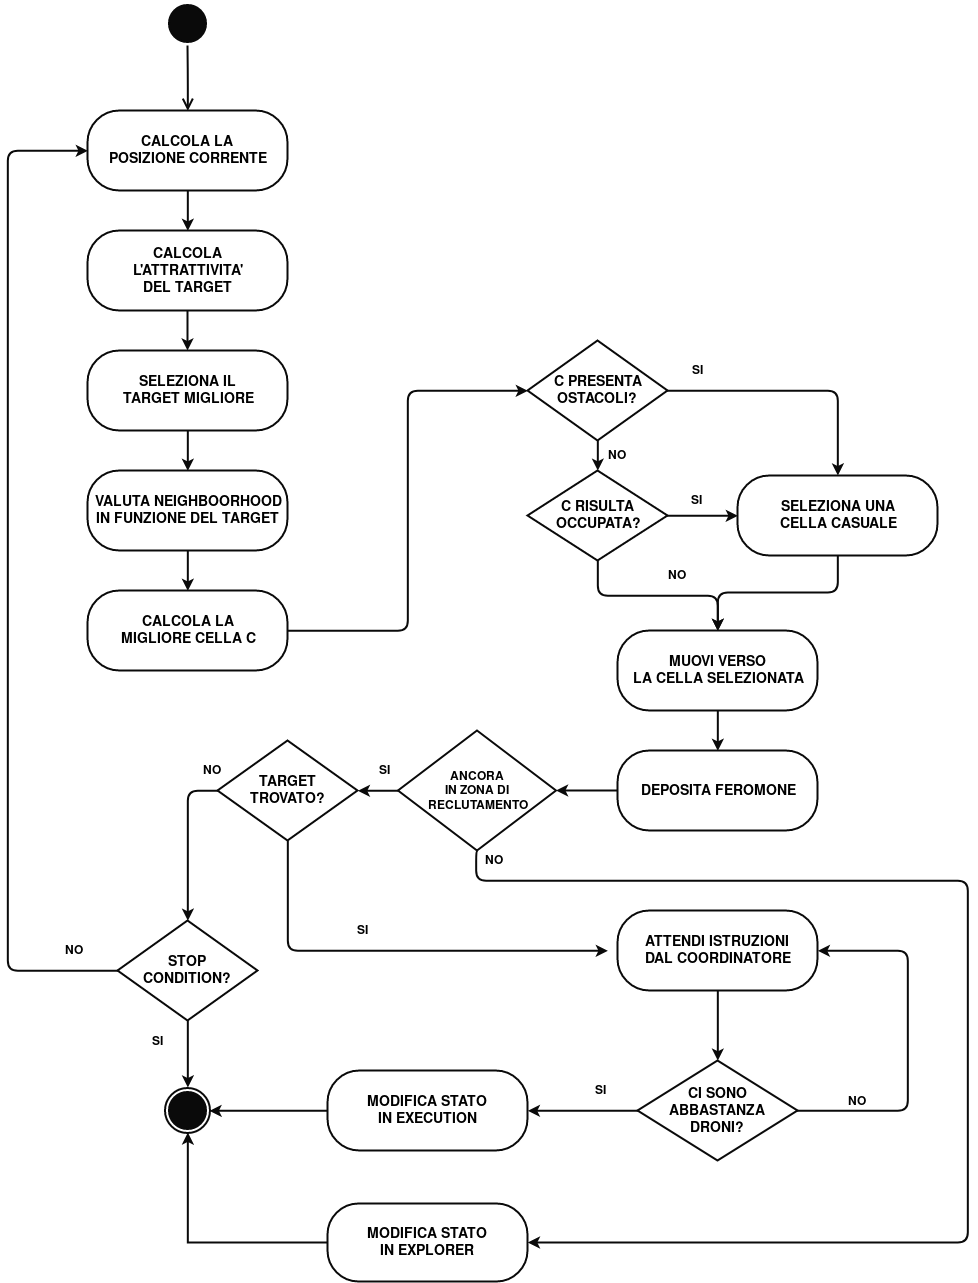
\includegraphics[width=0.5\paperwidth]{img/attivita_fts.png}}
    \end{center}
    \caption{Diagramma di attività per la strategia FTS-RR.}
    \label{attivita_fts}
\end{figure}

\paragraph{Strategia di reclutamento PSO-RR:} \textit{Particle Swarm Optimization} è una tecnica di ottimizzazione ispirata ai movimenti degli stormi.
Ogni agente $i$ si muove nello spazio di ricerca e presenta una velocità $v_{i}^{t}$ e delle coordinate $(x_{i}^{t},y_{i}^{t})$.
La velocità è aggiornata secondo la relazione seguente, in funzione delle coordinate di un target ricevute da un drone coordinatore:
\begin{equation}
    \begin{cases}
        v_{xi}^{t+1} = \omega v_{xi}^{t} + r \cdot c(x_{z} - x_{i}^{t}) \\
        v_{yi}^{t+1} = \omega v_{yi}^{t} + r \cdot c(y_{z} - y_{i}^{t})    
    \end{cases}    
\end{equation}
Dove:
\begin{itemize}
    \item $\omega$ è il coefficiente inerziale;
    \item $c$ è il coefficiente di accelerazione;
    \item $r \in [0,1]$ è un numero generato casualmente, per evitare blocchi in minimi locali.
\end{itemize}

Un drone $i$ che si trova nella cella di coordinate $(x_{i}^{t},y_{i}^{t})$, all'iterazione $t$, che riceve una richiesta d'aiuto da un coordinatore z, sceglierà la patch in cui muoversi secondo le seguenti espressioni:
\begin{equation}
    \begin{cases}
        x_{i}^{t+1} = x_{i}^{t} + 1 , \text{se}[v_{xi}^{t+1} > 0]\\
        x_{i}^{t+1} = x_{i}^{t} - 1 , \text{se}[v_{xi}^{t+1} < 0]\\
        x_{i}^{t+1} = x_{i}^{t} , \text{se}[v_{xi}^{t+1} = 0]
    \end{cases}
\end{equation}
e
\begin{equation}
    \begin{cases}
        y_{i}^{t+1} = y_{i}^{t} + 1 , \text{se}[v_{yi}^{t+1} > 0]\\
        y_{i}^{t+1} = y_{i}^{t} - 1 , \text{se}[v_{yi}^{t+1} < 0]\\
        y_{i}^{t+1} = y_{i}^{t} , \text{se}[v_{yi}^{t+1} = 0]
    \end{cases}
\end{equation}

Se il drone riceve richieste da più coordinatori, questo sceglierà di muoversi verso quello più vicino.

\begin{figure}[H] 
    \captionsetup{justification=centering, margin=2cm, font=footnotesize}
    \begin{center}
    \makebox[\textwidth]{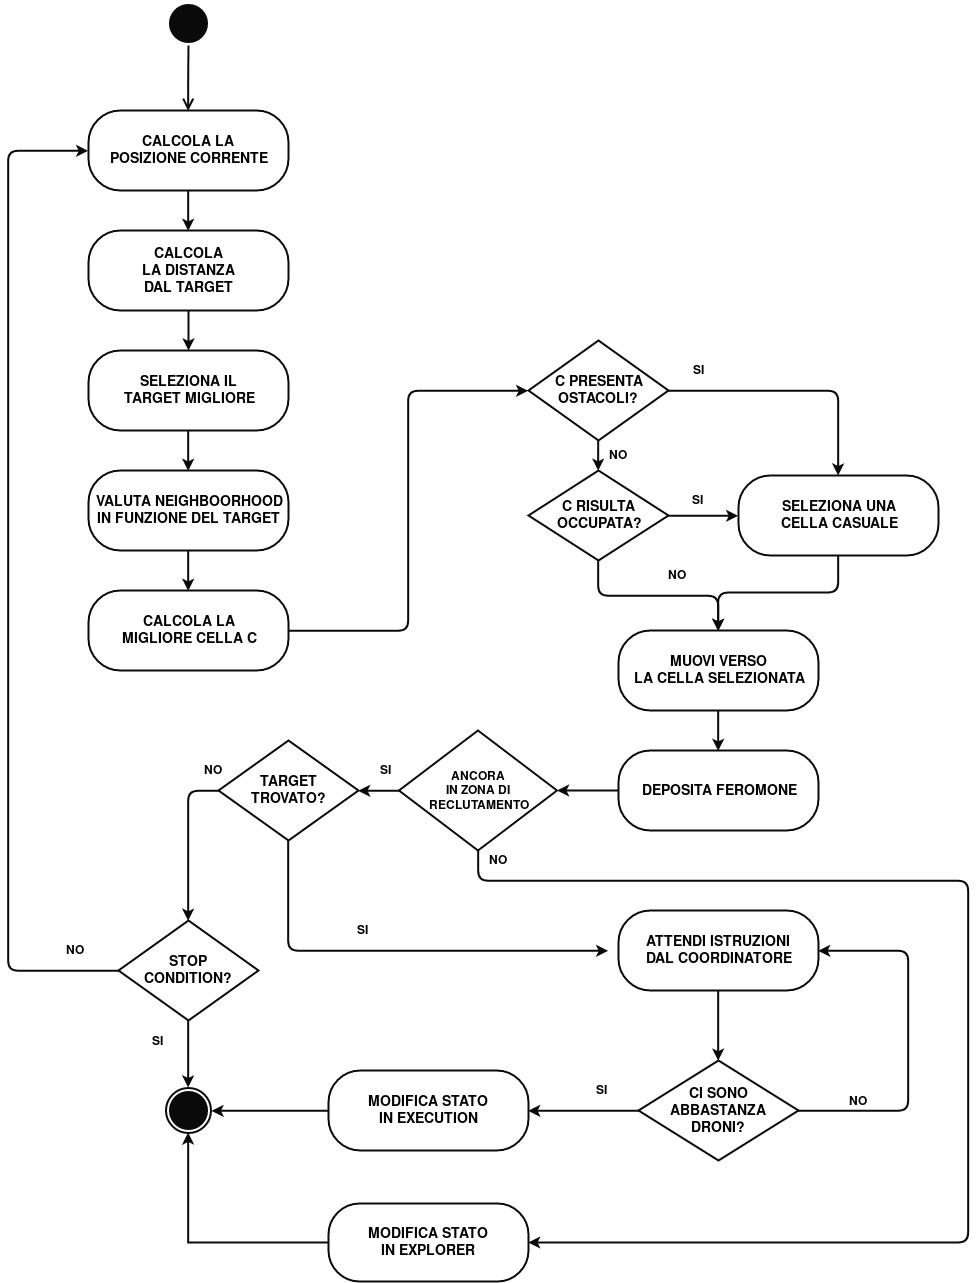
\includegraphics[width=0.5\paperwidth]{img/attivita_pso.png}}
    \end{center}
    \caption{Diagramma di attività per la strategia PSO-RR.}
    \label{attivita_pso}
\end{figure}

\paragraph{Strategia di reclutamento ABC-RR:} \textit{Artificial bee colony for robots recruitment} è una strategia che segue il comportamento delle api in cerca di una fonte di nutrimento di qualità. 
Nell’algoritmo in questione, la distribuzione di fonti di cibo, all’interno del territorio di esplorazione, può essere modificata dalle api stesse nel corso del tempo. 
L’algoritmo utilizza l’insieme delle api per trovare la soluzione ottima al problema. 

Nell'ambiente simulato, le fonti di cibo sono rappresentate dai target e la metaeuristica è applicata grazie alla comunicazione avviata dal coordinatore.

Sia $\phi \in [-1,1]$ un coefficiente scelto in modo casuale, ogni robot $i$ nel raggio di reclutamento di un coordinatore $z$, all'iterazione $t$, si muoverà in funzione delle seguenti equazioni:
\begin{equation}
    \begin{cases}
        x_{i}^{t+1} = x_{i}^{t} + \phi (x_{i}^{t} - x_{z}) \\
        y_{i}^{t+1} = y_{i}^{t} + \phi (y_{i}^{t} - y_{z})    
    \end{cases}    
\end{equation}

Se vogliamo applicare tali regole al piano bidimensionale dell'ambiente di simuazione, esse vanno adattate come segue:
\begin{equation}
    \begin{cases}
        x_{i}^{t+1} = x_{i}^{t} + 1 , \text{se}[\phi (x_{i}^{t} - x_{z}) > 0]\\
        x_{i}^{t+1} = x_{i}^{t} - 1 , \text{se}[\phi (x_{i}^{t} - x_{z}) < 0]\\
        x_{i}^{t+1} = x_{i}^{t} , \text{se}[\phi (x_{i}^{t} - x_{z}) = 0]
    \end{cases}
\end{equation}
e
\begin{equation}
    \begin{cases}
        y_{i}^{t+1} = y_{i}^{t} + 1 , \text{se}[\phi (y_{i}^{t} - y_{z}) > 0]\\
        y_{i}^{t+1} = y_{i}^{t} - 1 , \text{se}[\phi (y_{i}^{t} - y_{z}) < 0]\\
        y_{i}^{t+1} = y_{i}^{t} , \text{se}[\phi (y_{i}^{t} - y_{z}) = 0]
    \end{cases}
\end{equation}

Nel caso in cui un drone $i$ riceva più di una richiesta di aiuto, esso dovrà decidere quale coordinatore prendere come riferimento.
La \textit{qualità} di un coordinatore $z$ è definita come il reciproco della distanza:
\begin{equation}
    \mu_{z}^{i} = \frac{1}{r_{iz}}
\end{equation}
Dove $r_{iz}$ rappresenta la distanza euclidea tra $i$ e $z$.

La probabilità che il drone $i$ selezioni $z$ come coordinatore di riferimento è data da:
\begin{equation}
    p_{z}^{i} = P{coordinator_{i} = z} = \frac{\mu_{z}^{i}}{\sum_{b \in RR_{i}} \mu_{b}^{i}}
\end{equation}
Dove $RR_{i}$ è l'insieme di richieste di reclutamento ricevute da $i$.
In questo modo $\sum_{b \in RR_{i}} p_{b}^{i} = 1$.

Viene pertanto utilizzata la regola della \textit{spinning-wheel}: ad ogni coordinatore è associata una probabilità.
Se immaginiamo una \textit{ruota della fortuna}, possiamo rappresentare tale probabilità come una porzione più o meno grande  di questa ruota e la dimensione della porzione dipende proprio dalla probabilità calcolata.
Il drone farà girare questa ruota, in modo da ottenere il target (ed il coordinatore) di riferimento.

\begin{figure}[H] 
    \captionsetup{justification=centering, margin=2cm, font=footnotesize}
    \begin{center}
    \makebox[\textwidth]{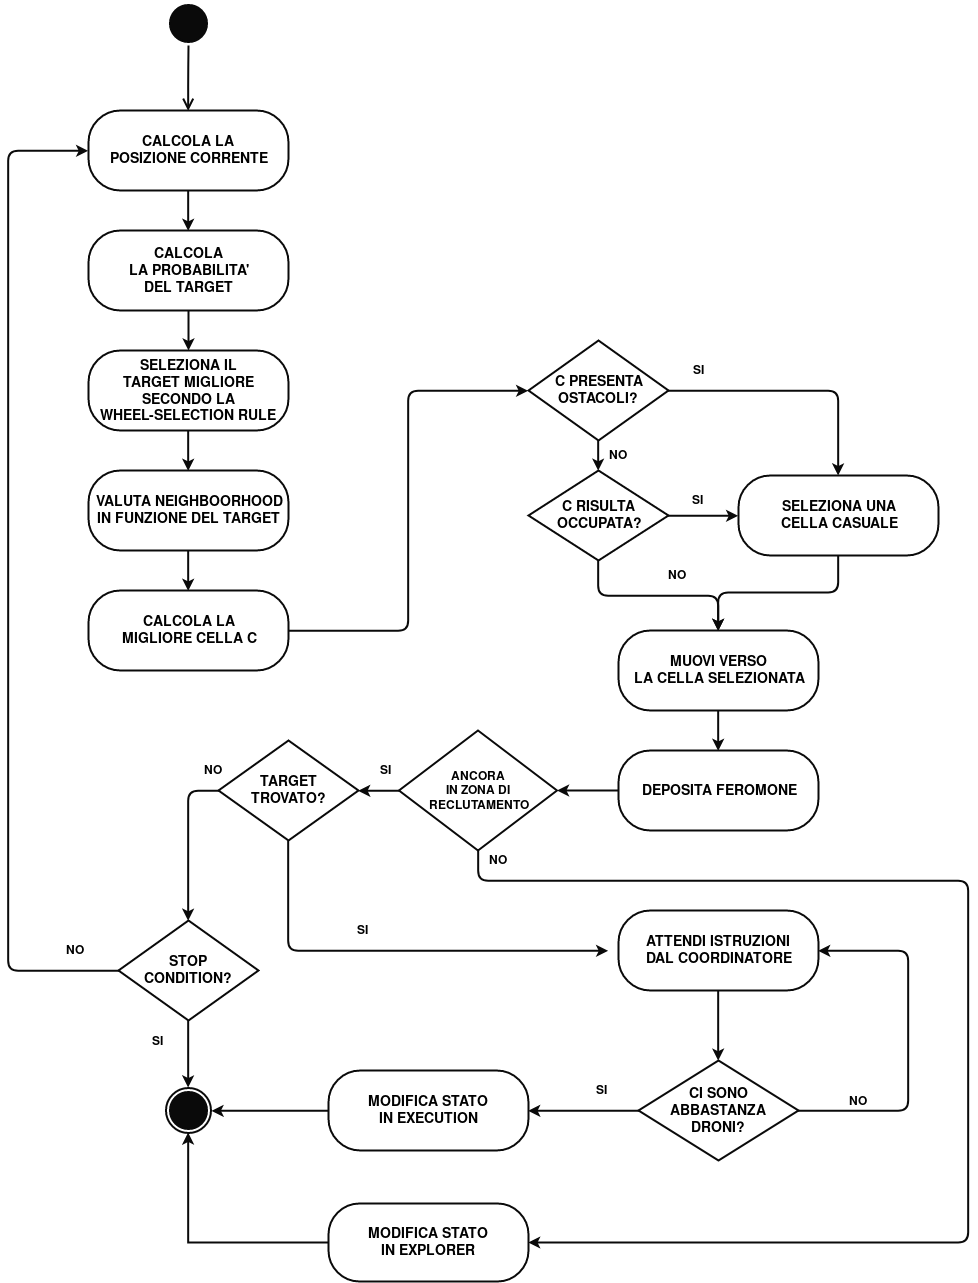
\includegraphics[width=0.5\paperwidth]{img/attivita_abc.png}}
    \end{center}
    \caption{Diagramma di attività per la strategia ABC-RR.}
    \label{attivita_abc}
\end{figure}